\documentclass[letterpaper,11pt,notitlepage]{article}
% define the title
\usepackage{amsmath}
\usepackage{fixltx2e}
\usepackage{graphicx}
\usepackage[labelformat=empty]{caption}
\usepackage{subcaption}
\usepackage{listings}
\usepackage{color}
\usepackage{relsize}
\usepackage{wrapfig}
\usepackage{fontspec}
\usepackage{hyperref}
\usepackage{hanging}
\usepackage{textcomp,    % for \textlangle and \textrangle macros
            xspace}
\newcommand\la{\textlangle}  % set up short-form macros
\newcommand\ra{\textrangle\xspace}
\newcommand\rans{\textrangle}
\lstset{
  language={matlab},
  basicstyle=\ttfamily\smaller\relax,	
  tabsize=4,                              % Default tab size
  % showspaces=false,                       % Dont make spaces visible
  showtabs=false,                         % Dont make tabls visible
  columns=flexible,                       % Column formatc
  commentstyle=\color{mygreen}\textit,           % comment style
  extendedchars=true,              % lets you use non-ASCII characters; for 8-bits encodings only, does not work with UTF-8
  numbers=left,                    % where to put the line-numbers; possible values are (none, left, right)
  numbersep=8pt,                   % how far the line-numbers are from the code
  numberstyle=\tiny\color{mygray}, % the style that is used for the line-numbers
  stepnumber=1,
  xleftmargin=2cm,
  % backgroundcolor=\color{light-gray},
  breaklines=true,
  keywordstyle=\color{mynavy}
}
\hypersetup{colorlinks=true,linkcolor=blue}
\renewcommand*{\UrlFont}{\ttfamily\smaller\relax}

% \addtolength{\oddsidemargin}{0.5in}
% \addtolength{\evensidemargin}{0.5in}
% \addtolength{\textwidth}{-1in}
\addtolength{\topmargin}{-1in}
\addtolength{\textheight}{1.75in}
\setlength\parindent{24pt}

% \author{Choong-Wan Woo}
% \title{Problem Set 1}
% \date{\today}

\definecolor{mygreen}{rgb}{0.1020,0.5961,0.3137}
\definecolor{mygray}{rgb}{0.5,0.5,0.5}
\definecolor{light-gray}{rgb}{0.8,0.8,0.8}
\definecolor{mynavy}{rgb}{0.1922,0.2118,0.5843}

\begin{document}

\begin{center}
	Homework 1 - KNN\\
	2015 Spring, Machine Learning\\
	Choong-Wan Woo\\
	\today\\
\end{center}

\hspace*{-1cm}\textbf{Analysis 1.}  \rule{10.5cm}{0.4pt}\\
\noindent\textit{What is the role of the number of training points to accuracy?}\\

\noindent As you can see in \textbf{Figure}, as the number of training points (\textit{n} in Figure) increase, the accuracy increases. 
\begin{figure}[ht!]
	\centering
	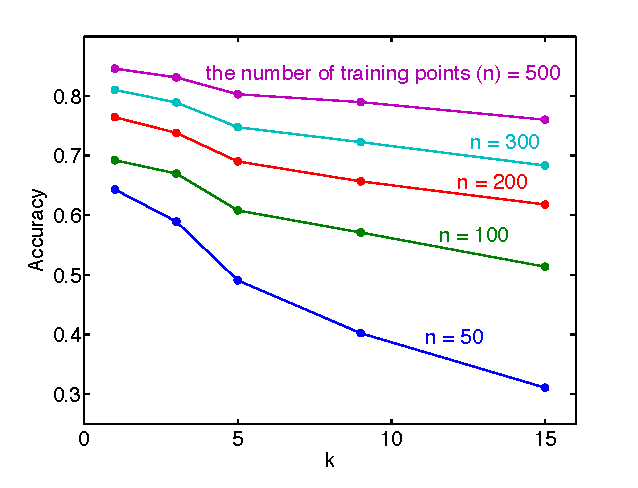
\includegraphics[width=7.5cm]{figure1_legend}
	\captionsetup{width=.8\textwidth}
	\caption{\textbf{Figure.} The analysis results. X-axis represents the number of nearest neighbors (\textit{k}), and y-axis represents accuracy calculated from the confusion matrix. Different lines show tests with different numbers of training points.}
\end{figure}\\

\hspace*{-1cm}\textbf{Analysis 2.}  \rule{10.5cm}{0.4pt}\\
\noindent\textit{What is the role of k to accuracy?}\\

\noindent As \textbf{Figure} demonstrate, the \textit{k} increases, the accuracy decreases.\\\\

\hspace*{-1cm}\textbf{Analysis 3.}  \rule{10.5cm}{0.4pt}\\
\noindent\textit{What numbers get confused with each other most easily?}\\

\noindent From my testing space (i.e., \textit{k} = [1,3,5,9,15], and \textit{n} = [50,100,200,300,500]), \textbf{7 and 9} were the pair that yielded the largest number of errors. 

\end{document}